\begin{frame}{RAM - What is it?}
\begin{columns}
    \begin{column}{0.47\textwidth}
    \begin{block}{RAM}
        \begin{itemize}
            \item Volatile 
            \item Fast
            \item Low latency
            \item Expensive
        \end{itemize}
    \end{block}
    \end{column}
    \begin{column}{0.47\textwidth}
        \begin{figure}
        \centering
        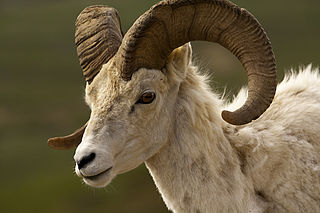
\includegraphics[width=\textwidth]{img/ram.jpg}
        \caption{Not this}
        \label{fig:my_label}
    \end{figure}
    \end{column}
\end{columns}
\end{frame}
\begin{frame}{RAM - Why we are interested}
    \begin{block}{Reasons}
        \item Transient data
        \item Fast
    \end{block}
\end{frame}
\note{When dealing with Transient data it shouldn't be stored in main memory if it can be avoided as this slows down the process.} 
\begin{frame}{RAM - How to access it?}
    \begin{block}{In a file system}
        \begin{itemize}
            \item Mount it in a directory
            \item Use a temporary file system, i.e tmpfs
            \item mount -t tmpfs -o size=8G tmpfs /mnt/ram
        \end{itemize}
    \end{block}
    \begin{block}{In object storage (Ceph)}
        \begin{itemize}
            \item Well its not as easy. 
        \end{itemize}
    \end{block}
\end{frame}
\note{It is quite simple, you would create a directory such as /mnt/ram and then apply a temporary file system to it. An wallah you have access to RAM in a file storage way.}
